186. \begin{figure}[ht!]
\center{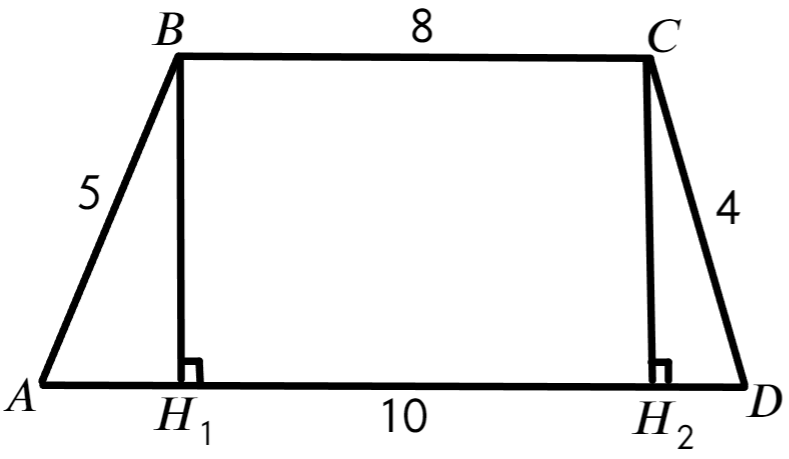
\includegraphics[scale=0.35]{g9-186.png}}
\end{figure}\\
Опустим высоты $BH_1=CH_2=h.$ Пусть $AH_1=x,$ тогда $H_2D=10-8-x=2-x$ и и по теореме Пифагора для треугольников $ABH_1$ и $CDH_2$ имеем равенства $h^2=25-x^2=16-(2-x)^2,$ откуда $25-x^2=16-4+4x-x^2,\ 4x=13,\ x=\cfrac{13}{4}.$ Тогда $h^2=25-\cfrac{169}{16}=\cfrac{231}{16},\ h=\cfrac{\sqrt{231}}{4}.$ Пусть расстояние от точки $C$ до прямой $AB$ равно $h_1.$ Посчитаем площадь треугольника $ABC$ двумя способами: $\cfrac{1}{2}\cdot\cfrac{\sqrt{231}}{4}\cdot8=
\cfrac{1}{2}\cdot h_1\cdot5,\ h_1=\cfrac{2\sqrt{231}}{5}.$\\
